\documentclass[compress]{beamer}
\usepackage{ifthen,verbatim}

\newcommand{\isnote}{}
\xdefinecolor{lightyellow}{rgb}{1.,1.,0.25}
\xdefinecolor{darkblue}{rgb}{0.1,0.1,0.7}

%% Uncomment this to get annotations
%% \def\notes{\addtocounter{page}{-1}
%%            \renewcommand{\isnote}{*}
%% 	   \beamertemplateshadingbackground{lightyellow}{white}
%%            \begin{frame}
%%            \frametitle{Notes for the previous page (page \insertpagenumber)}
%%            \itemize}
%% \def\endnotes{\enditemize
%% 	      \end{frame}
%%               \beamertemplateshadingbackground{white}{white}
%%               \renewcommand{\isnote}{}}

%% Uncomment this to not get annotations
\def\notes{\comment}
\def\endnotes{\endcomment}

\setbeamertemplate{navigation symbols}{}
\setbeamertemplate{headline}{\mbox{ } \hfill
\begin{minipage}{5.5 cm}
\vspace{-0.75 cm} \small
\end{minipage} \hfill
\begin{minipage}{4.5 cm}
\vspace{-0.75 cm} \small
\begin{flushright}
\ifthenelse{\equal{\insertpagenumber}{1}}{}{ \hspace{0.2 cm} \insertpagenumber\isnote/\pageref{numpages}}
\end{flushright}
\end{minipage} \hspace{0.01 cm} \vspace{-1.05 cm}}

\newcommand{\s}[1]{{\mbox{\scriptsize #1}}}

\begin{document}
\begin{frame}
\vfill
\begin{center}
\textcolor{darkblue}{\Large Why do we need a Higgs boson?}

\vfill
\begin{columns}
\column{0.3\linewidth}
\begin{center}
\large
Jim Pivarski
\end{center}
\end{columns}

%% \begin{columns}
%% \column{0.3\linewidth}
%% \begin{center}
%% \scriptsize
%% {\it Fermilab}
%% \end{center}
%% \end{columns}

\vfill
 8 December, 2011

\end{center}
\end{frame}

%% \begin{notes}
%% \item This is the annotated version of my talk.
%% \item If you want the version that I am presenting, download the one
%% labeled ``slides'' on Indico (or just ignore these yellow pages).
%% \item The annotated version is provided for extra detail and a written
%% record of comments that I intend to make orally.
%% \item Yellow notes refer to the content on the {\it previous} page.
%% \item All other slides are identical for the two versions.
%% \end{notes}

\small

\begin{frame}
\frametitle{My background}

CMU physics major, class of '99 \\\vspace{0.3 cm}
Worked with an electron-positron collider at Cornell as a graduate student, measured the $\Upsilon$ wavefunction for a Ph.D.\ thesis in 2006 \\\vspace{0.3 cm}
Postdoc at Texas A\&M until this year, worked on the CMS experiment at the Large Hadron Collider (LHC); searched for exotic particles in the early data (``muonic jets''--- didn't see any) \\\vspace{0.3 cm}

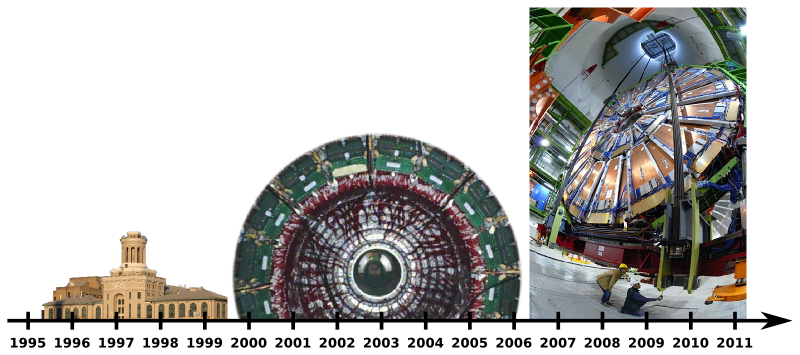
\includegraphics[width=\linewidth]{timeline.png}
\end{frame}

\begin{frame}
\frametitle{My background}

\vspace{-0.75 cm} \hfill 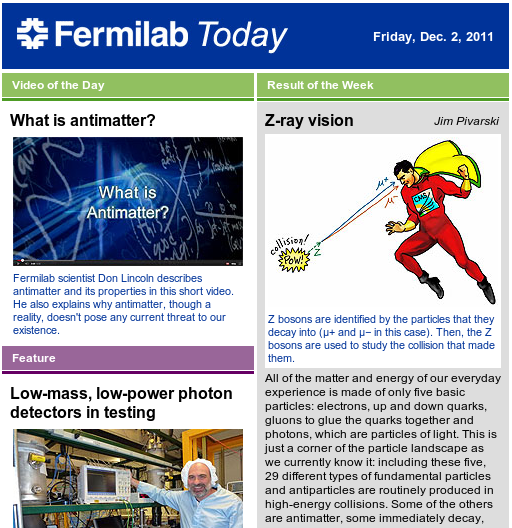
\includegraphics[width=4 cm]{fermilab_today.png}

\vspace{-3.5 cm}
This year, I've completely changed course: \\\vspace{0.1 cm}
\hspace{0.5 cm} now I do part-time work in industry \\
\hspace{1 cm} as a statistician/programmer \\
\hspace{0.5 cm} and use my free time to write popular \\
\hspace{1 cm} physics articles, make outreach \\
\hspace{1 cm} demonstrations and presentations

\vfill
\hspace{-0.83 cm} \textcolor{darkblue}{\Large What is this talk about?}

\vspace{0.3 cm}
The most difficult thing to explain is the significance of the Higgs boson
\begin{itemize}
\item the ``origin of mass'' story neglects the fact that most mass (protons, dark matter) is not due to the Higgs mechanism
\item an explanation of electroweak symmetry breaking requires a more sophisticated audience
\end{itemize}

In this talk, I'll explain why the Higgs mechanism is important, drawing on your background in intro quantum and intermediate E\&M
\end{frame}

\begin{frame}
\frametitle{Cartoon of quantum field theory}

Imagine a space-filling field, like the electric field, but instead of having a set of numbers (a vector) at each point in space, we have an amplitude function (whose square is a probability distribution) at each point

\vspace{0.3 cm}
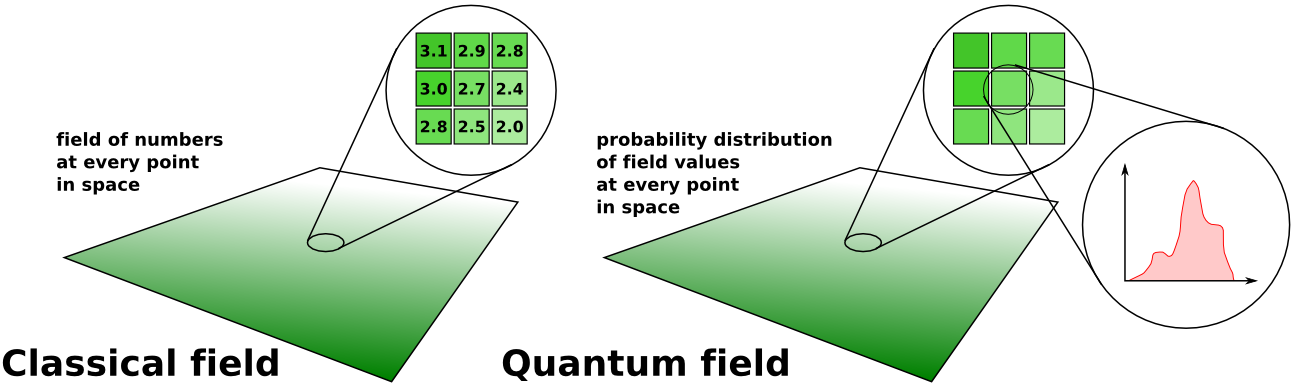
\includegraphics[width=\linewidth]{classical_quantum_fields.png}

\vspace{0.3 cm}
\begin{itemize}
\item This picture combines the field concept from E\&M with the indeterminacy of quantum mechanics
\item It provides our current best-understanding of particles and forces
\end{itemize}
\end{frame}

\begin{frame}
Schr\"odinger equation for field value $\phi$ at a space-time point $(t, \vec{x})$:

\[ i \sqrt{\left( \frac{\partial \Psi}{\partial t} \right)^2 - \nabla^2 \Psi} = \left( -\frac{1}{2} \frac{\partial^2}{\partial \phi^2} + V(\phi) \right) \Psi(\phi; t, \vec{x}) \]

\vspace{-0.25 cm}
{\scriptsize \hspace{2.4 cm} propagation \hspace{1.1 cm} kinetic \hspace{0.22 cm} potential }

\vspace{-0.2 cm}
{\scriptsize \hspace{5.2 cm} energy \hspace{0.35 cm} energy }

\vspace{0.2 cm}
where $\Psi$ is the amplitude function over field value $\phi$

\vfill
\hspace{-0.83 cm} \textcolor{darkblue}{\Large Particles in quantum field theory}

\begin{columns}
\column{0.5\linewidth}

Parabolic potential: $\displaystyle V(\phi) = \frac{1}{2} m^2 \phi^2$

It costs energy to make field

\vspace{0.5 cm}
Solve by separating $\phi$ dependence from space-time dependence:

\vspace{-0.4 cm}
\[ \Psi(\phi; t, \vec{x}) = \psi(\phi) \varphi(t, \vec{x}) \]
\column{0.5\linewidth}
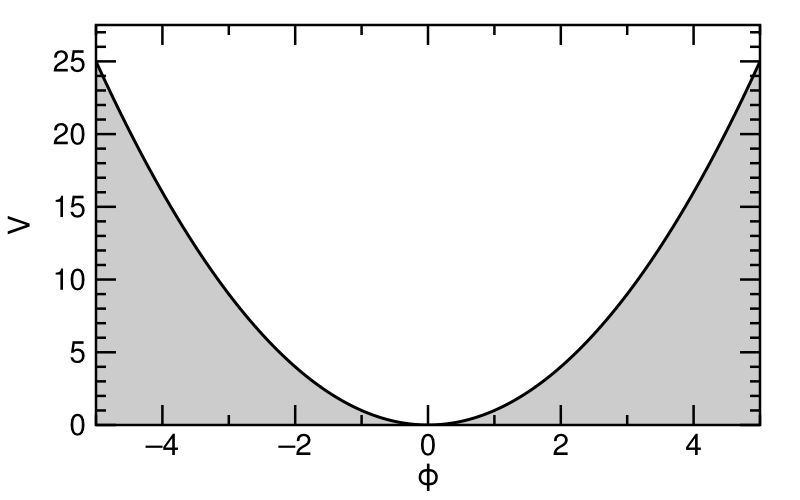
\includegraphics[width=\linewidth]{potential_quadratic.png}
\end{columns}

\mbox{$\displaystyle \frac{i}{\varphi(t, \vec{x})} \sqrt{\left( \frac{\partial \varphi}{\partial t} \right)^2 - \nabla^2 \varphi} = -\frac{1}{2\psi(\phi)} \left( \frac{\partial^2}{\partial \phi^2} - m^2 \phi^2 \psi(\phi) \right) = \mbox{a constant } M$\hspace{-1 cm}}

\hfill \textcolor{darkblue}{\scriptsize \it (continued\ldots)}
\end{frame}

\begin{frame}
{\scriptsize \it (repeat from previous page\ldots)}

\mbox{$\displaystyle \frac{i}{\varphi(t, \vec{x})} \sqrt{\left( \frac{\partial \varphi}{\partial t} \right)^2 - \nabla^2 \varphi} = -\frac{1}{2\psi(\phi)} \left( \frac{\partial^2}{\partial \phi^2} - m^2 \phi^2 \psi(\phi) \right) = \mbox{a constant } M$\hspace{-1 cm}}

\vfill
The left-hand side is solved by plane waves:

\vspace{-0.3 cm}
\[ \varphi(t, \vec{x}) = \mbox{constant} \times \exp(iEt + i\vec{p} \cdot \vec{x}) \mbox{ with } \sqrt{E^2 - |\vec{p}|^2} = M \]

\vfill
The right-hand side is a hard equation to satisfy:
% \[ (m^2 \phi^2 - 2 M) \psi(\phi) = \frac{\partial^2 \psi}{\partial \phi^2} \]

\vspace{-0.3 cm}
\[ \psi(\phi) = \mbox{constant} \times \exp(-\tfrac{1}{2} m \phi^2) H_n(\sqrt{m} \phi) \]

where $H_n$ are Hermite polynomials and $M = (n + \tfrac{1}{2}) m$ for integers $n \ge 0$.

\vspace{0.3 cm}
This is why particles are particulate: the rest energy of a field is quantized into a zero-particle solution, a one-particle solution, etc.

\vfill
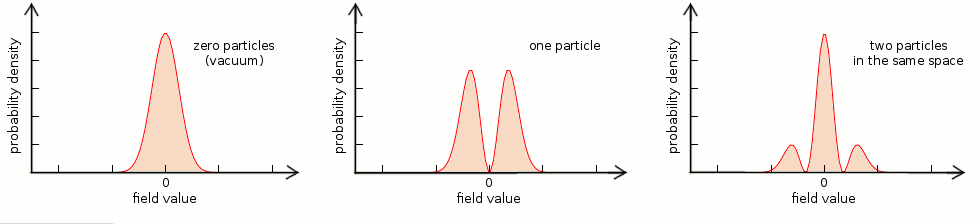
\includegraphics[width=\linewidth]{fieldvalues.png}
\end{frame}

\begin{frame}
\hfill 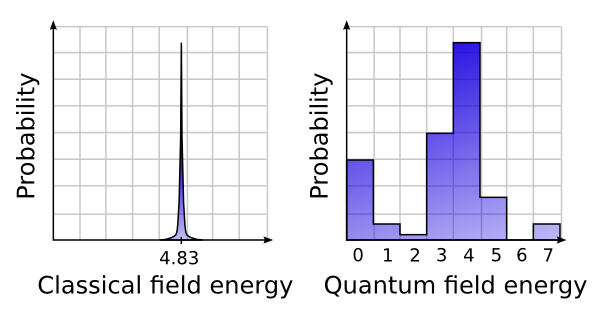
\includegraphics[width=0.5\linewidth]{quantum_field_energy.png}

\vspace{-2.8 cm}
Quantum field theory is both more \\ constrained and less constrained \\ than classical field theory:
\begin{itemize}
\item the rest energy is constrained \\ to be a multiple of an integer
\item but solutions can superimpose
\end{itemize}

It explains why energy comes in chunks called particles, and it does so in a framework that allows particles to be created and destroyed

\vspace{0.3 cm}
\mbox{ } \hfill 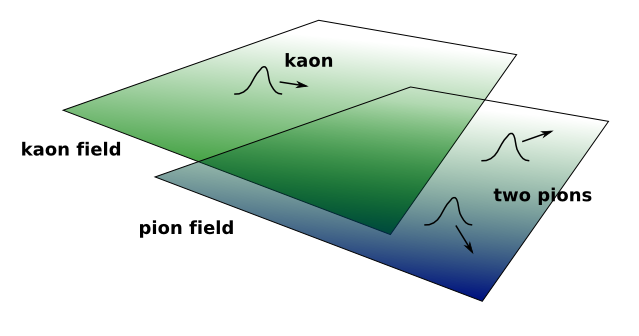
\includegraphics[width=0.55\linewidth]{ktopipi_fields.png} \hfill \mbox{ }

\vspace{-0.3 cm}
For example, when a kaon decays into two pions, an excitation of the kaon field is transferred to two excitations of the pion field because the kaon field is coupled to the pion field by a $(c \, \phi_K \phi_\pi)$ term in the potential
\end{frame}

\begin{frame}


\begin{columns}
\column{0.35\linewidth}
\begin{center}
Bubble chamber photo

\vspace{0.1 cm}
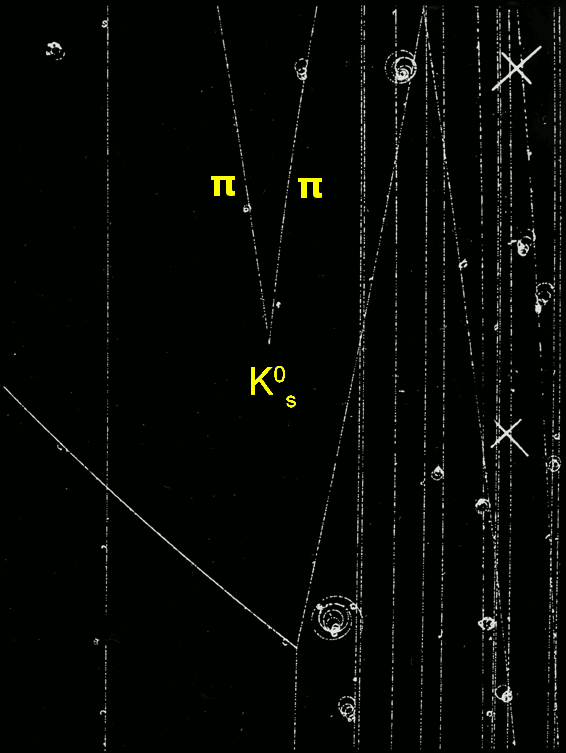
\includegraphics[height=4.5 cm]{k0-to-pipi_bubblechamber.png}

\vspace{0.1 cm}
\scriptsize proton beam (upward) on liquid containing protons (stationary)
\end{center}

\column{0.65\linewidth}
\begin{center}
Reconstructed LHC event

\vspace{0.1 cm}
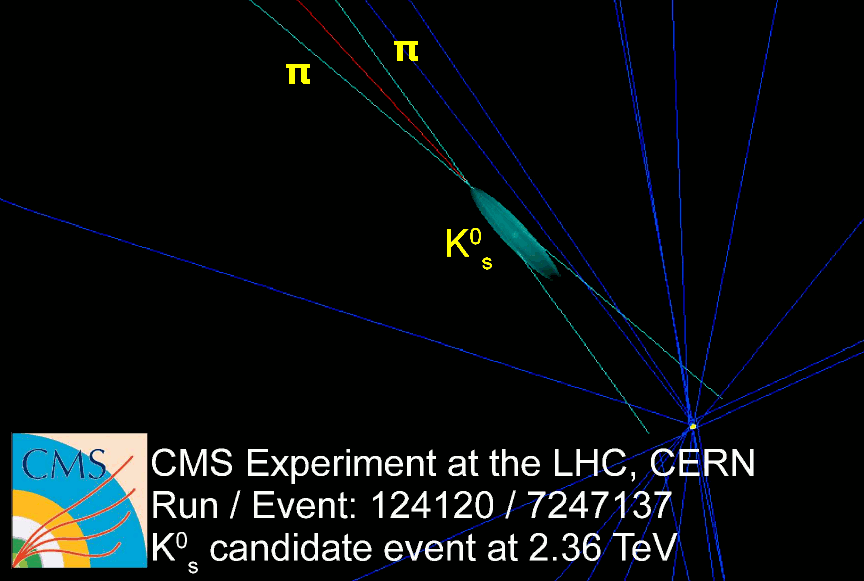
\includegraphics[height=4.5 cm]{cms_kshort.png}

\vspace{0.1 cm}
\scriptsize incoming proton beams are perpendicular to this projection, collide at a point and outgoing particles radiate in all directions
\end{center}

\end{columns}

\uncover<2>{\vspace{-3.3 cm} \hfill \begin{minipage}{5 cm} 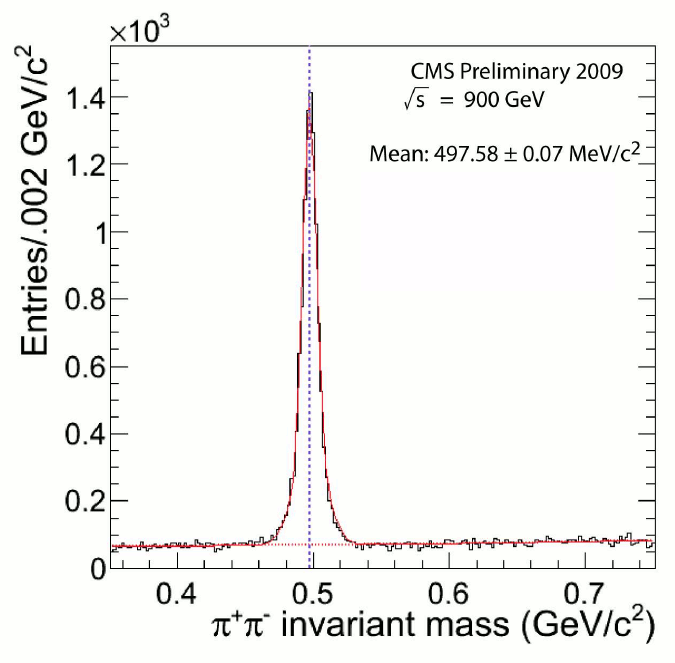
\includegraphics[height=5 cm]{kshort-distribution.png} \\ \mbox{$\sqrt{E^2 - |\vec{p}|^2} = \mbox{ that constant } M$\hspace{-1 cm}} \end{minipage}}
\end{frame}

\begin{frame}
\frametitle{Forces are a consequence of symmetry}

If we want a model's Lagrangian (kinetic energy minus potential energy) to be independent of the complex phase of its fields,

\vspace{-0.1 cm}
\[ \phi(t, \vec{x}) \to e^{i \alpha(t, \vec{x})} \phi(t, \vec{x}) \]

\vspace{0.1 cm}
then we must add another field $A(t, \vec{x})$ to enforce this symmetry

\begin{itemize}
\item $\phi(t, \vec{x})$ is the field of any charged particle (e.g.\ electrons)
\item the invariance $\alpha(t, \vec{x})$ is ``gauge freedom'' from E\&M
\item and $A(t, \vec{x})$ is the electromagnetic field (a.k.a.\ photons)
\end{itemize}

But the photon field cannot have a mass term $\displaystyle \frac{1}{2} {m_\gamma}^2 |A|^2$, since that would violate the symmetry

\vfill
1940/50's: Quantum field theory with phase symmetry {\it implies} the existence of electromagnetic forces with no photon mass.  Light {\it must} be.

Q.E.D.
\end{frame}

\begin{frame}
\frametitle{The Standard Model (except for Higgs)}

All known forces except gravity can be described as a single quantum field theory with a (somewhat more complicated) symmetry principle

\begin{center}
\renewcommand{\arraystretch}{1.2}
\begin{tabular}{c c c}
electromagnetic & photon & massless \\\hline
strong nuclear & gluons (8 kinds) & massless \\
{\scriptsize holds protons together} & & \\\hline
weak nuclear & $W^+$, $W^-$, $Z$ & $m_{W^\pm} = 80.40 \pm 0.02$~GeV \\
{\scriptsize slow radioactive decays} & & $m_{Z} = 91.188 \pm 0.002$~GeV \\
\end{tabular}

\vspace{-0.5 cm}
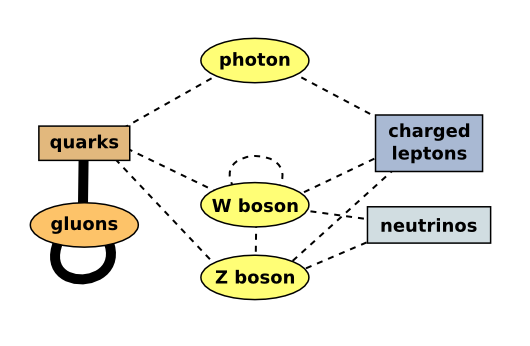
\includegraphics[width=0.7\linewidth]{standard_model.png}
\end{center}

\vspace{-1.3 cm}
\hfill {\scriptsize lines indicate couplings}
\end{frame}

\begin{frame}
\frametitle{\mbox{ } \hfill \hfill \LARGE The Problem \hfill \mbox{ }}

\Large

The symmetry principle explains the existence of all of the forces--- photon, gluons, $W^\pm$ and $Z$--- in one nice package

\vfill
But $W^\pm$ and $Z$ are not massless; they violate the symmetry principle!
\end{frame}

\begin{frame}
\frametitle{\mbox{The Englert-Brout-Higgs-Guralnik-Hagen-Kibble field\hspace{-1 cm}}}

\begin{columns}
\column{0.01\linewidth}

\column{0.5\linewidth}
1964: Consider adding a field $\phi_H$ with the following potential:

\vspace{-0.1 cm}
\[ V(\phi_H) = \mu^2 |\phi_H|^2 + \lambda |\phi|^4 \]

\vspace{0.1 cm}
where $\mu^2$ is {\it negative.}

\column{0.5\linewidth}
\only<1>{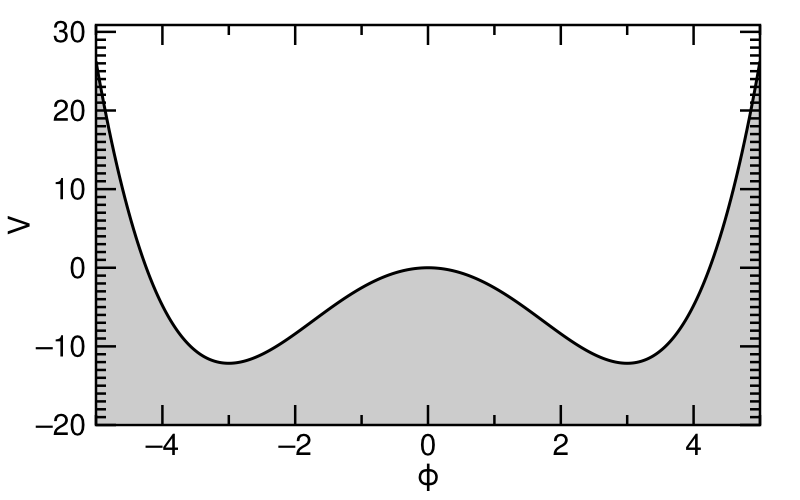
\includegraphics[width=\linewidth]{potential_mexicanhat.png}}
\only<2>{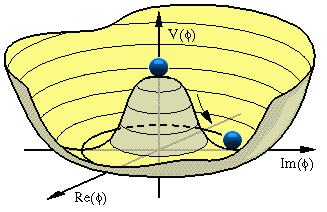
\includegraphics[width=\linewidth]{higgs-mecanisme.png}}
\end{columns}

The ground state solution is peaked at one of the minima, where $\displaystyle \phi_H = \sqrt{-\mu^2/\lambda} = \nu \approx \frac{1}{\sqrt{\mbox{246 GeV}}}$, rather than at $\phi_H = 0$

\begin{itemize}
\item Space would be filled field values near $\nu$: the Higgs condensate
\item The particle potentials we observe are perturbations around $\nu$, not the potentials in the fundamental theory
\item The Higgs field itself has an approximately parabolic potential around $\nu$: the Higgs boson
\end{itemize}
\end{frame}

\begin{frame}
\frametitle{Generating effective masses}

\renewcommand{\arraystretch}{1.2}
\begin{tabular}{c c}
\vspace{-0.1 cm} fundamental theory & \vspace{-0.1 cm} effective theory \\
& {\scriptsize (expansion around $\phi_H = \nu$)} \\\hline
no explicit $W$ or $Z$ mass terms & \\
symmetry generates forces & \\
\vspace{-0.06 cm} \uncover<2->{Higgs-$W$ and Higgs-$Z$ interactions} & \vspace{-0.06 cm}\uncover<2->{look like $W$ and $Z$ mass terms} \\
\uncover<3->{e.g.\ coupling term $ig\phi_W\phi_H$} & \uncover<3->{becomes $(g\nu)^2 |\phi_W|^2$ at $\phi_H = \nu$} \\
\vspace{-0.06 cm} \uncover<4->{Higgs interacts with} & \vspace{-0.06 cm} \uncover<4->{also look like mass terms} \\
\uncover<4->{charged leptons and quarks} & \\
\end{tabular}

\vspace{-0.5 cm}
\only<1>{\hfill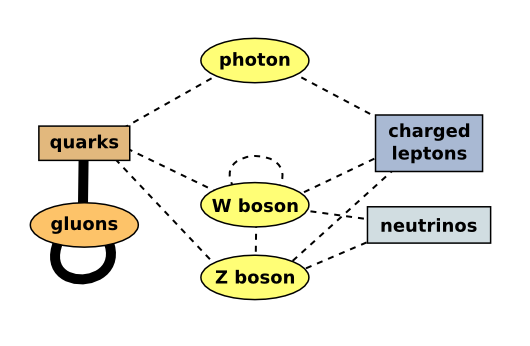
\includegraphics[width=0.65\linewidth]{standard_model.png}}
\only<2-3>{\hfill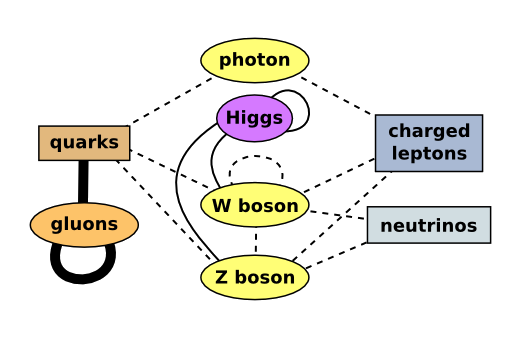
\includegraphics[width=0.65\linewidth]{standard_model_whiggs.png}}
\only<4>{\hfill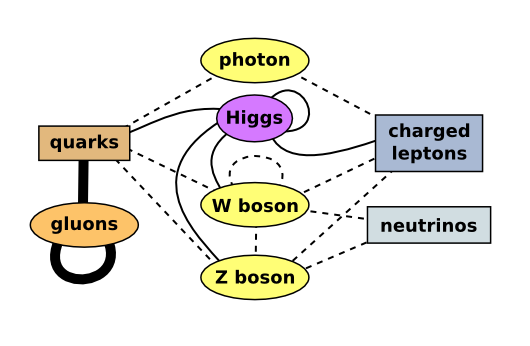
\includegraphics[width=0.65\linewidth]{standard_model_whiggs_quarkmass.png}}
\vspace{-0.75 cm}
\end{frame}

%% \begin{frame}
%% \frametitle{Generating effective masses}

%% Particles without symmetry-breaking mass terms can acquire an effective mass by interacting with the omnipresent Higgs condensate

%% \vspace{-1 cm}
%% \begin{center}
%% \renewcommand{\arraystretch}{1.5}
%% \begin{tabular}{c c c}
%% \vspace{-0.08 cm} & \vspace{-0.08 cm} & \vspace{-0.08 cm} re-expressed \\
%% \vspace{-0.08 cm} & \vspace{-0.08 cm} interaction term & \vspace{-0.08 cm} in coordinates \\
%% & & centered on $\phi_H = \nu$ \\\hline
%% between $W$ and Higgs & $ig\phi_W\phi_H$ & $(g\nu)^2 |\phi_W|^2$ \\
%% between $A$, $B$ and Higgs & $ig'\phi_A\phi_H + ig'\phi_B\phi_H$ & $(g + g')\nu^2 |\phi_Z|^2$ \\
%% & & + $0 \times |\phi_{\mbox{\scriptsize photon}}|^2$ \\
%% \uncover<3>{charged leptons and Higgs} & \uncover<3>{$g_e (\phi_{e_L} \phi_H \phi_{e_R} + \mbox{c.c.})$} & \uncover<3>{$\tfrac{1}{2} (g_e \nu)^2 |\phi_e|^2$} \\
%% \end{tabular}

%% \vspace{-0.3 cm}
%% \only<1>{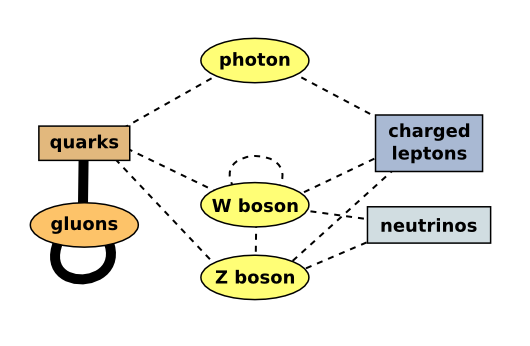
\includegraphics[width=0.65\linewidth]{standard_model.png}}
%% \only<2>{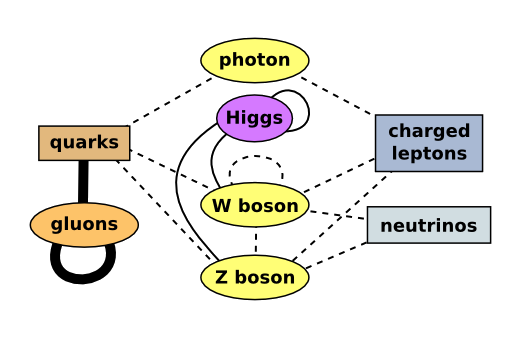
\includegraphics[width=0.65\linewidth]{standard_model_whiggs.png}}
%% \only<3>{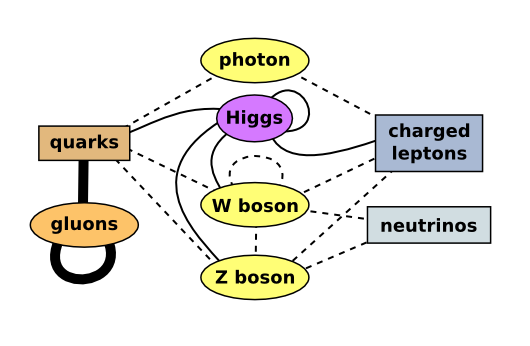
\includegraphics[width=0.65\linewidth]{standard_model_whiggs_quarkmass.png}}
%% \end{center}
%% \vspace{-1.5 cm}
%% \end{frame}

%% \begin{frame}
%% Introducing the Higgs field makes the Standard Model a consistent theory

%% \vfill
%% It is an extremely accurate description of nature
%% \begin{itemize}
%% \item of the thousands of measurements made since its development in the late 1960's, very few cast doubt on the Standard Model
%% \end{itemize}

%% \vfill
%% Many alternative theories have Higgs-like particles (composite Higgs made of more fundamental particles, multiple Higgses, etc.)

%% \vfill
%% Therefore, we strongly believe that something plays the role of a Higgs and gives $W$, $Z$, charged leptons, and quarks their effective masses
%% \end{frame}

\begin{frame}
Introducing the Higgs field makes the Standard Model a consistent theory

\vfill
\mbox{ } \hfill But is it true? \hfill \mbox{ }

\vfill
Standard Model was formulated around 1972--1976 and has been tested ever since.  Example of precision:
\begin{center}
\begin{tabular}{c c c}
& experiment & theory \\\hline
$m_{W}$ & $80.40 \pm 0.02$~GeV & $80.39 \pm 0.02$~GeV \\
$m_{Z}$ & $91.188 \pm 0.002$~GeV & $91.187 \pm 0.002$~GeV \\
\end{tabular}
\end{center}

\vfill
The only part that hasn't been observed is the Higgs boson, the one-particle excitation of the Higgs field around $\phi_H = \nu$
\end{frame}

\begin{frame}
\frametitle{Searching for the Higgs boson}
\textcolor{darkblue}{Popular Mechanics, April 1978}
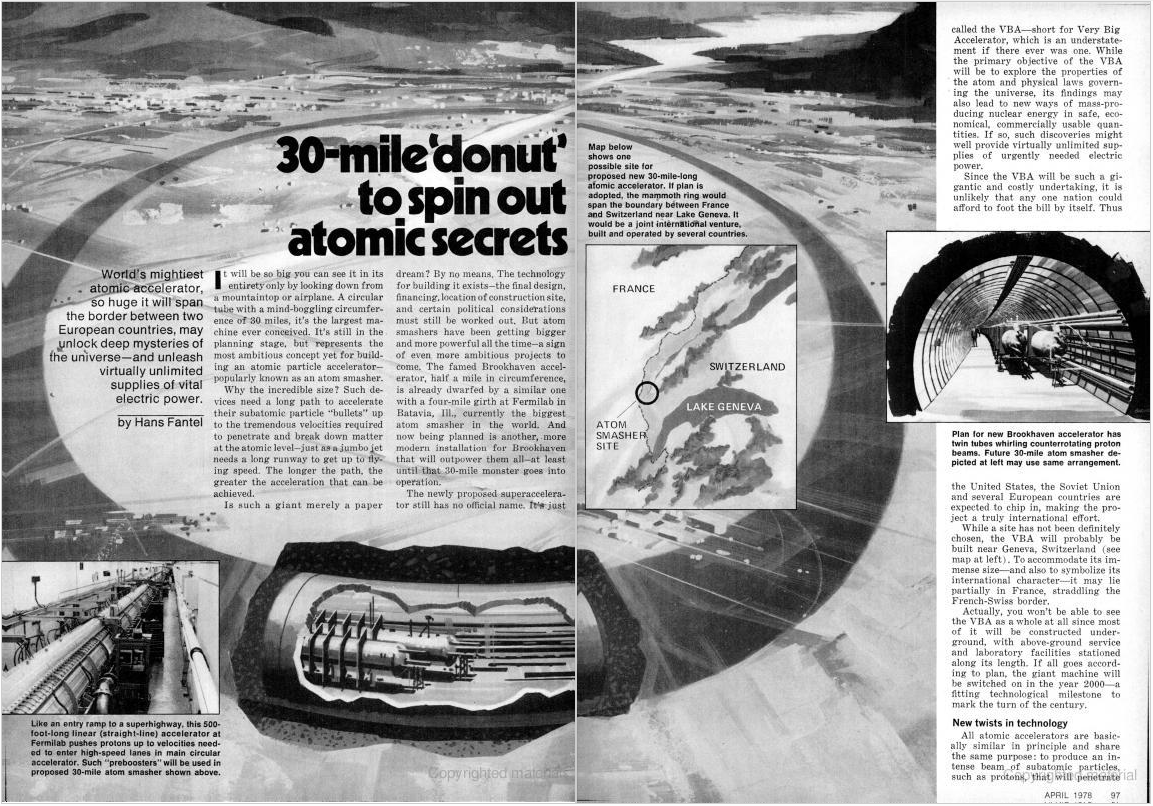
\includegraphics[width=\linewidth]{popular_mechanics.png}
\end{frame}

\begin{frame}
\frametitle{Searching for the Higgs boson}
\begin{center}
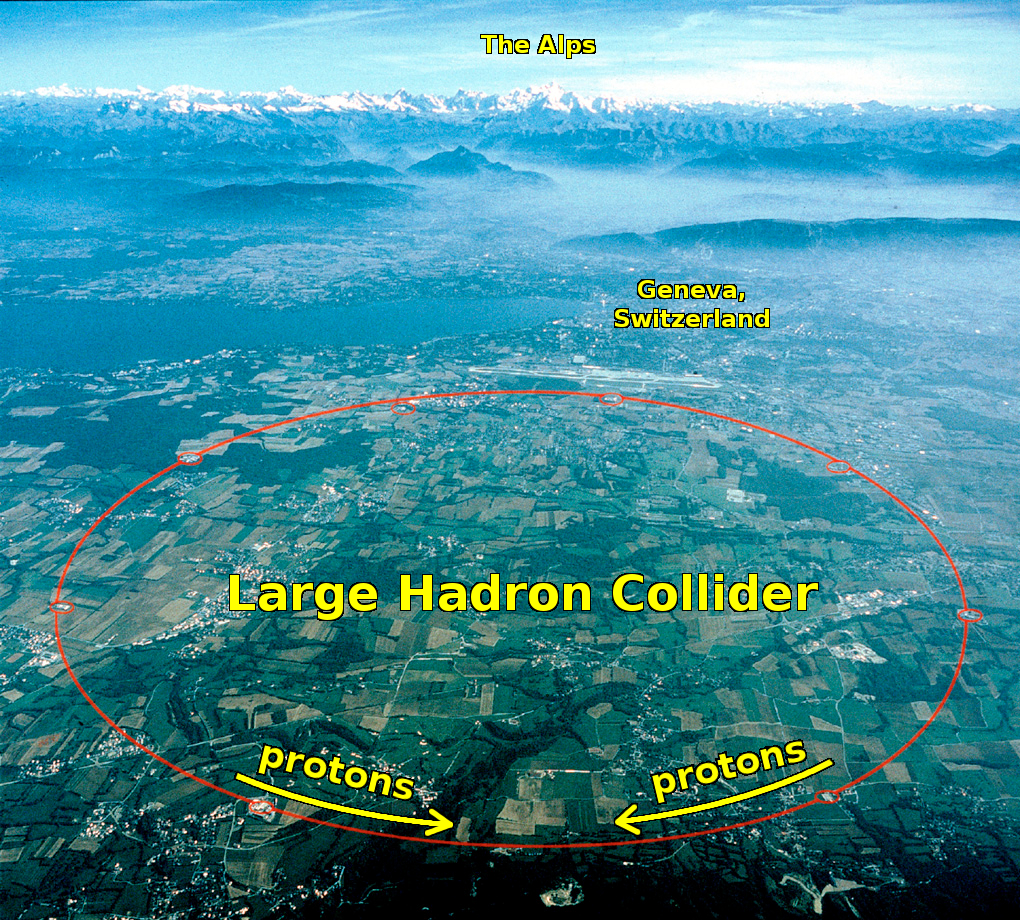
\includegraphics[width=0.8\linewidth]{cernpanorama.jpg}
\end{center}
\end{frame}

\begin{frame}
\vspace{0.5 cm}
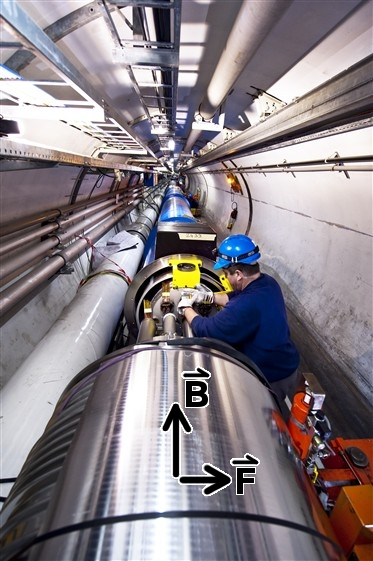
\includegraphics[height=6 cm]{lhc_dipole.jpg} \hfill
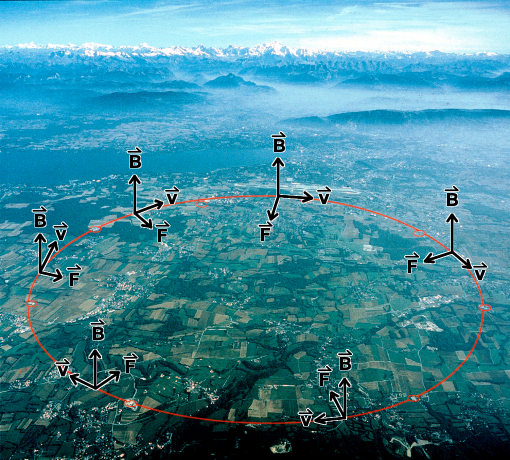
\includegraphics[height=6 cm]{cernpanorama_bfield.jpg} \hfill
\begin{itemize}
\item Protons confined by strong magnetic field ($\vec{F} = q\vec{v} \times \vec{B}$)
\begin{itemize}
\item ultra-high current solenoids made from superconducting wires
\end{itemize}

\item Protons accelerated by oscillating electric fields
\begin{itemize}
\item timed such that bunches of protons enter the field only when they're pointing the right way
\end{itemize}
\end{itemize}
\end{frame}

\begin{frame}
\frametitle{ATLAS on the Swiss side of the ring}

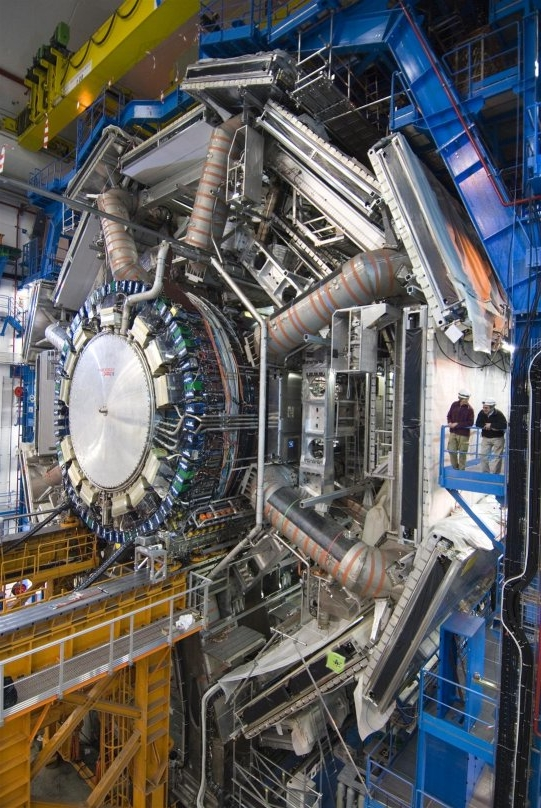
\includegraphics[height=5.1 cm]{atlas2.jpg} \hspace{0.2 cm}
\mbox{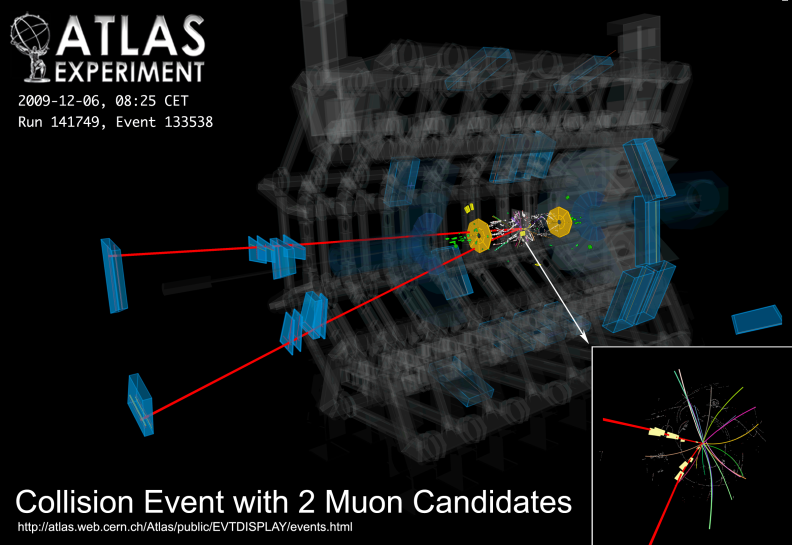
\includegraphics[height=5.1 cm]{atlas_dimuon.png} \hspace{-1 cm}}

\vfill
\uncover<2>{\mbox{ } \hfill 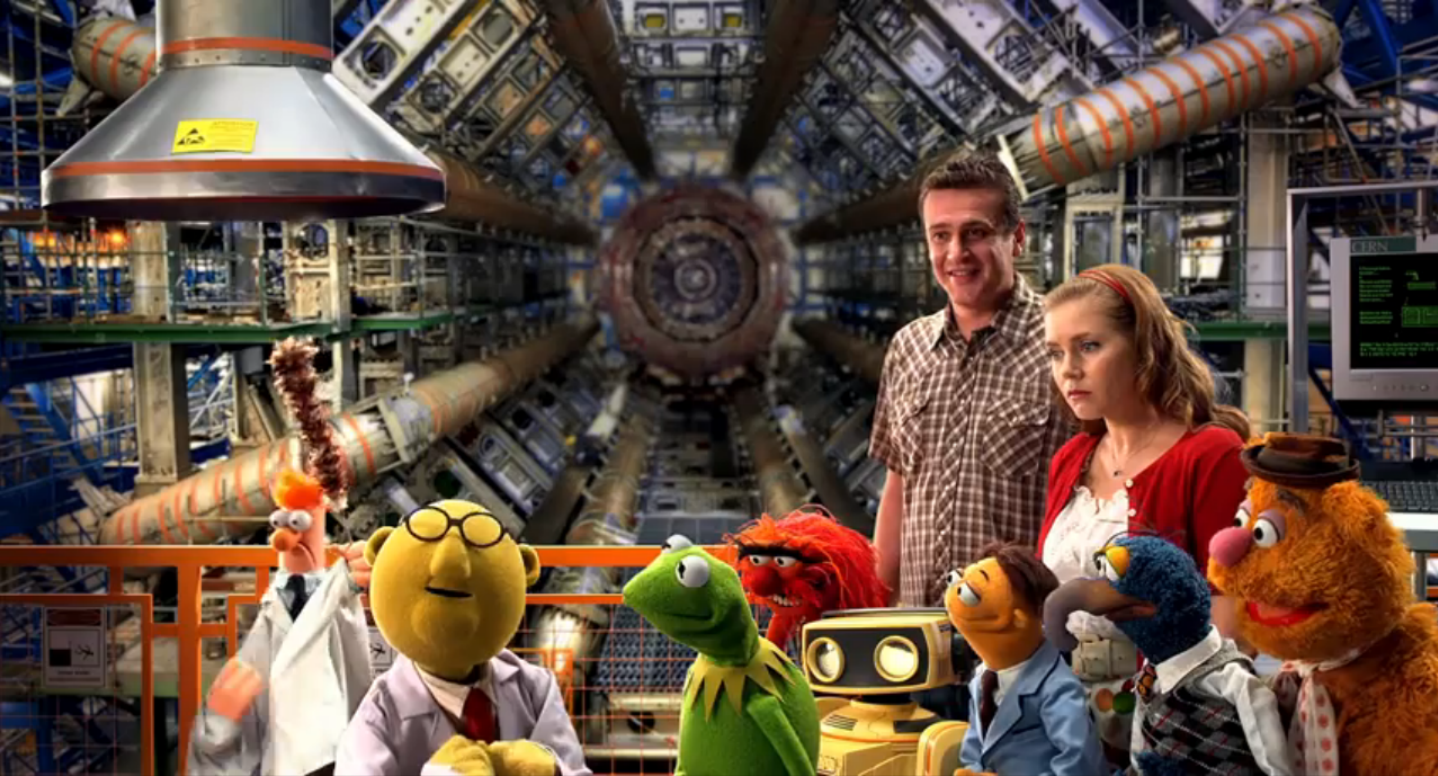
\includegraphics[height=3 cm]{muppets.png} \hspace{0.2 cm}
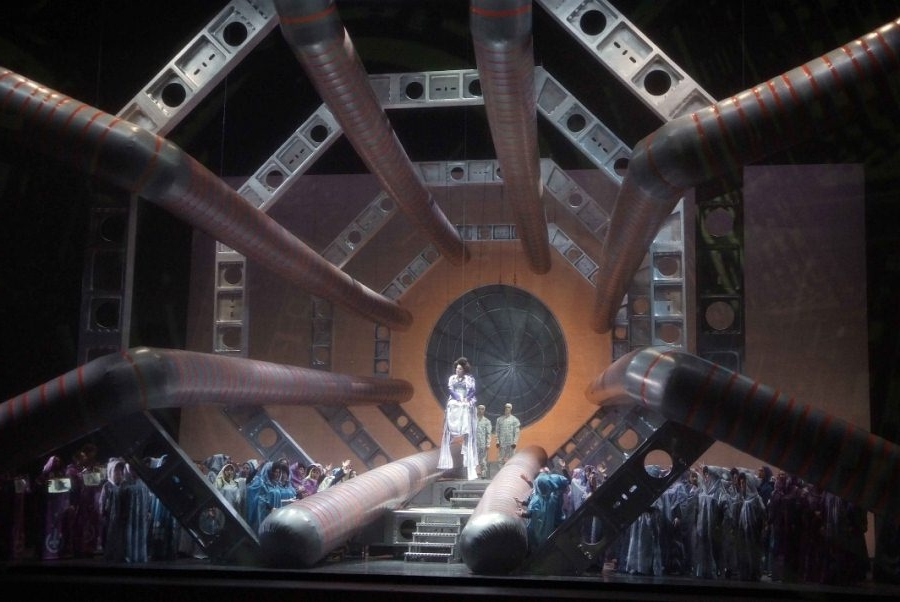
\includegraphics[height=3 cm]{berlioz_troyens.jpg} \hfill \mbox{ }}
\end{frame}

\begin{frame}
\frametitle{CMS on the French side of the ring}

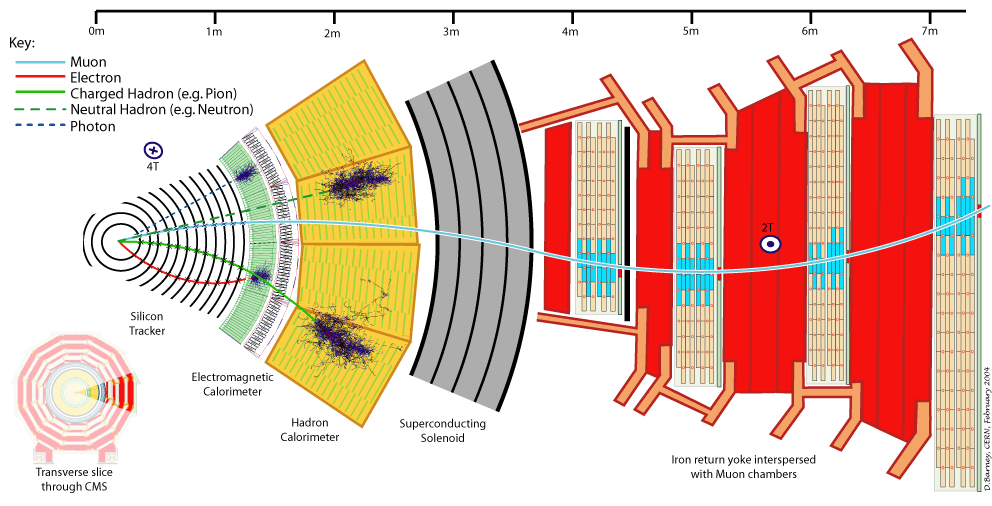
\includegraphics[height=3.5 cm]{cms_particles.png} 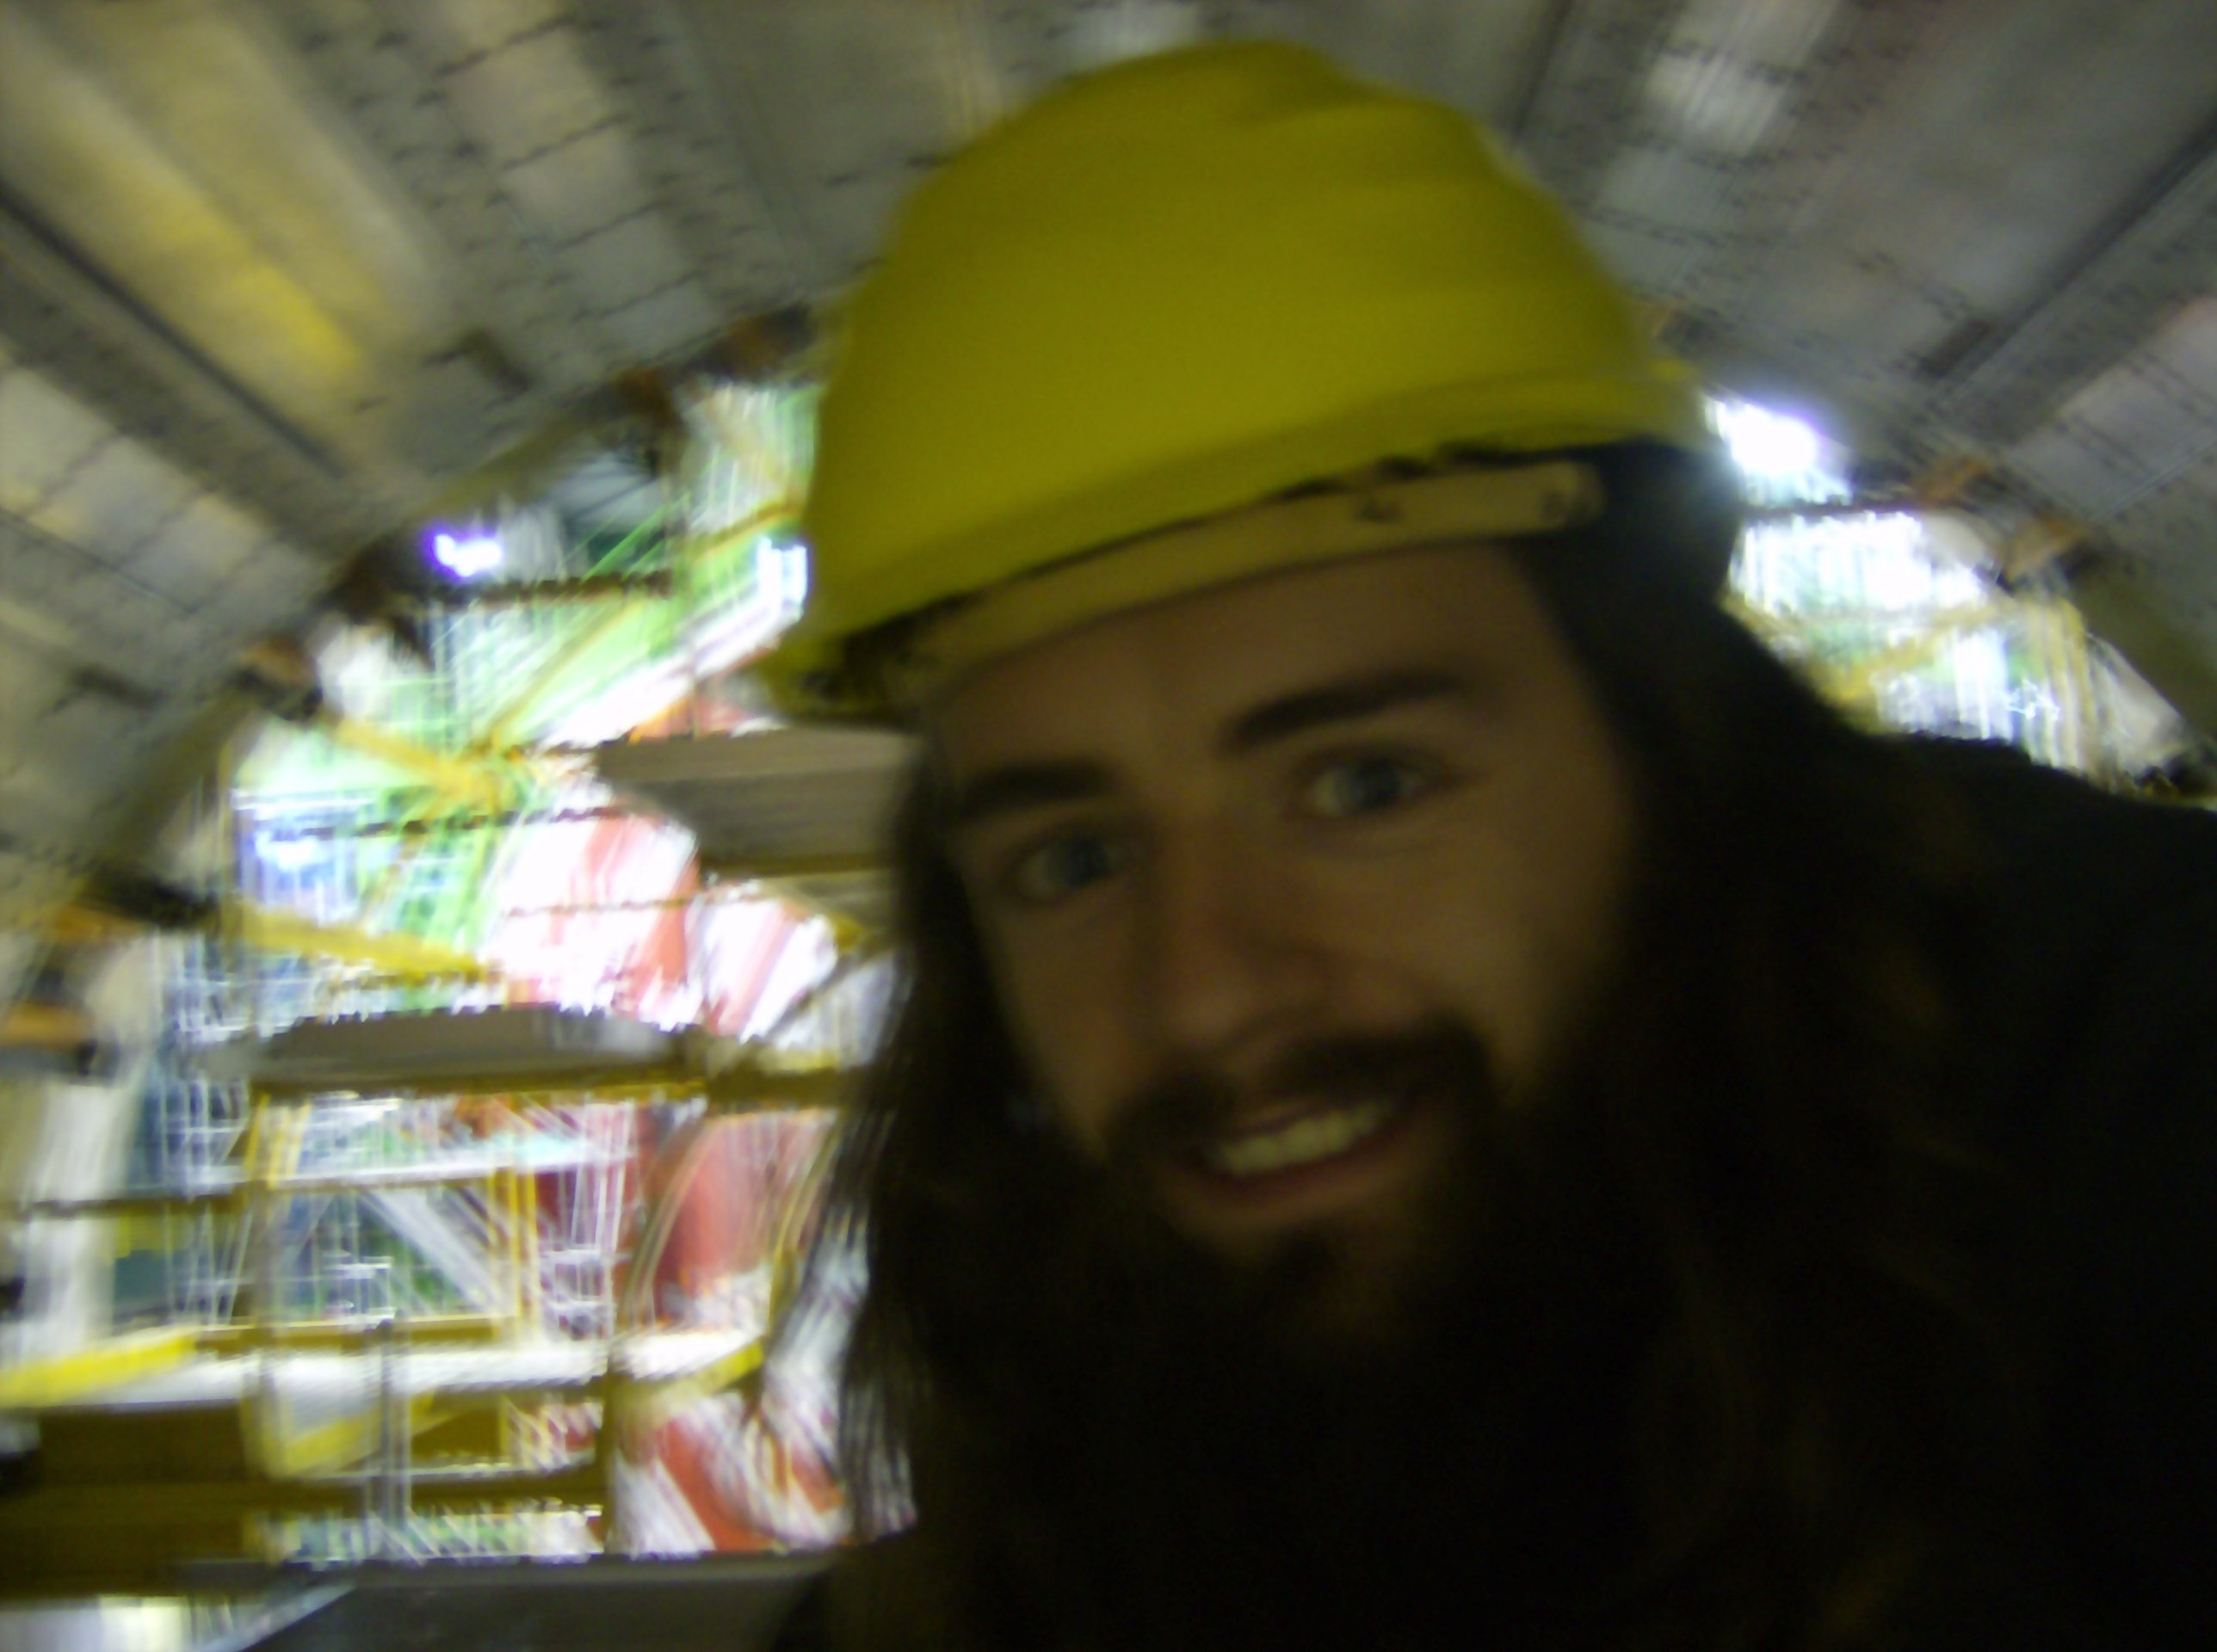
\includegraphics[height=3.5 cm]{hpim0592_SMILE.jpg}

\vfill

\mbox{\hspace{-0.4 cm}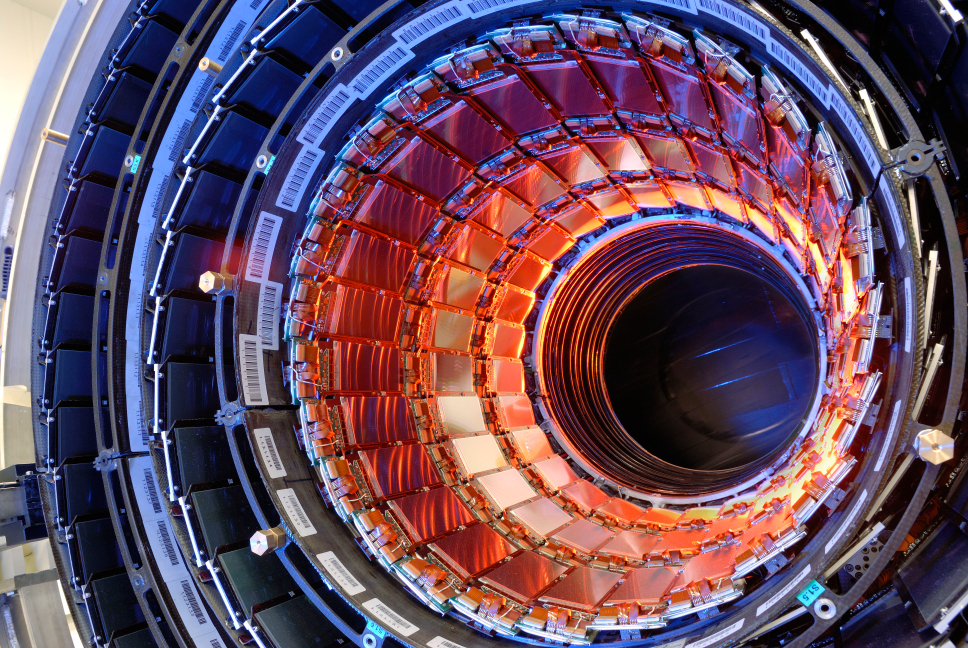
\includegraphics[height=4.1 cm]{tracker.jpg}} \hspace{0.1 cm}
\mbox{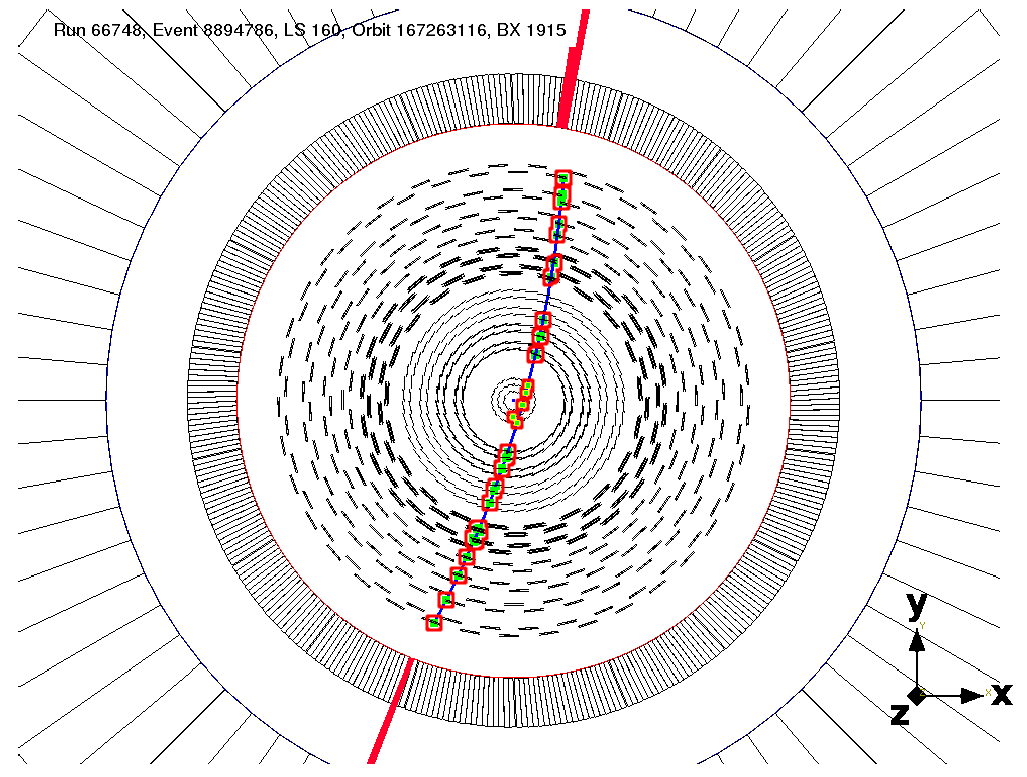
\includegraphics[height=4.1 cm]{cosmic_event.png} \hspace{-1 cm}}

\end{frame}

\begin{frame}
\frametitle{What we know from Higgs searches}
\begin{itemize}
\item Dozens of different decay signatures, most are hard to distinguish from other Standard Model processes
\item To get enough statistical significance, all of these analyses are combined into a single upper-limit plot
\item Also (sometimes) combine experiments
\end{itemize}

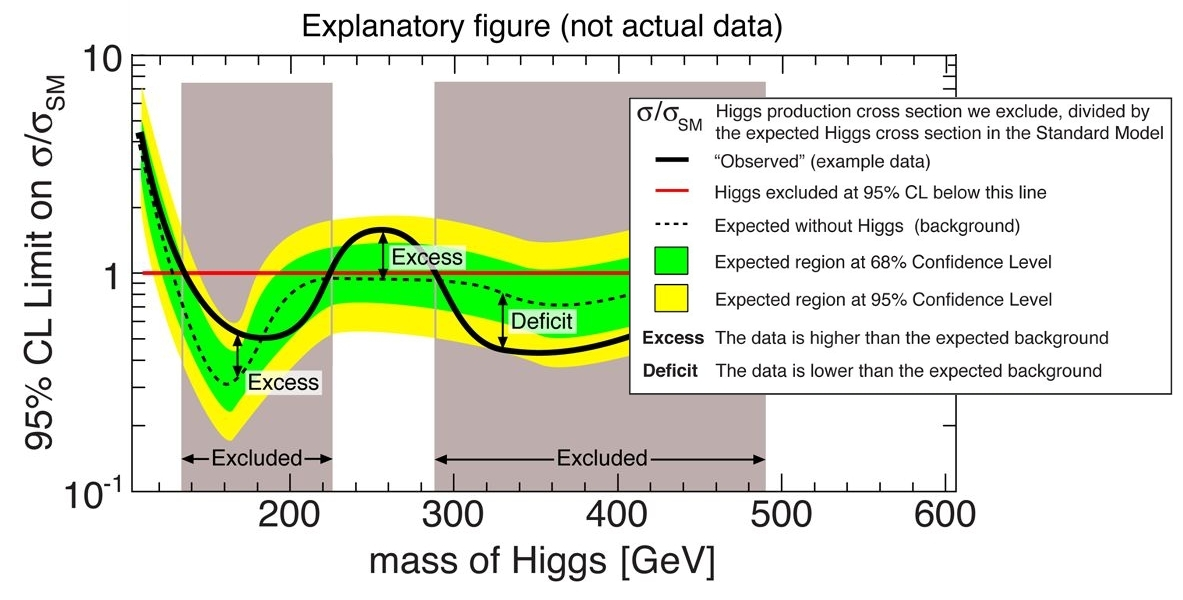
\includegraphics[width=\linewidth]{explaination_limitplot3.jpg}
\end{frame}

\begin{frame}
\frametitle{ATLAS + CMS combination, not full dataset}
\only<1>{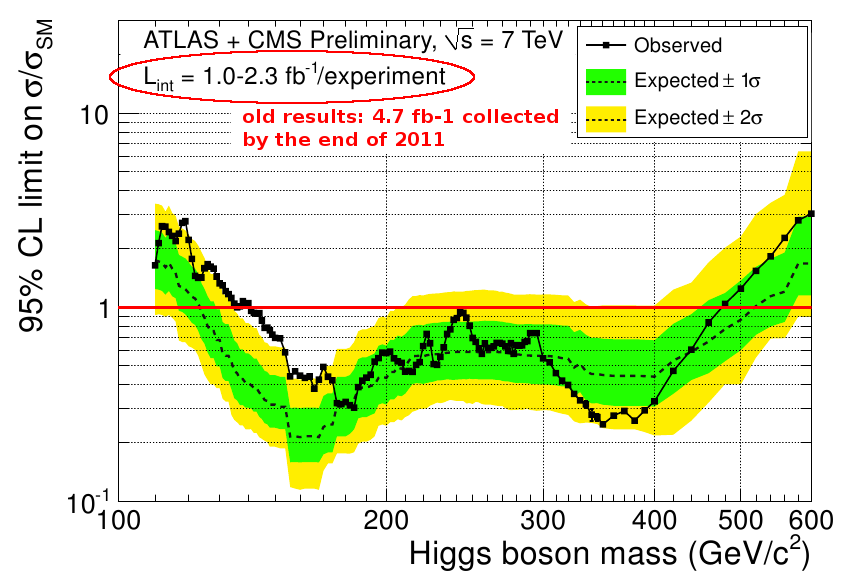
\includegraphics[width=\linewidth]{higgs_limits.png}}
\only<2>{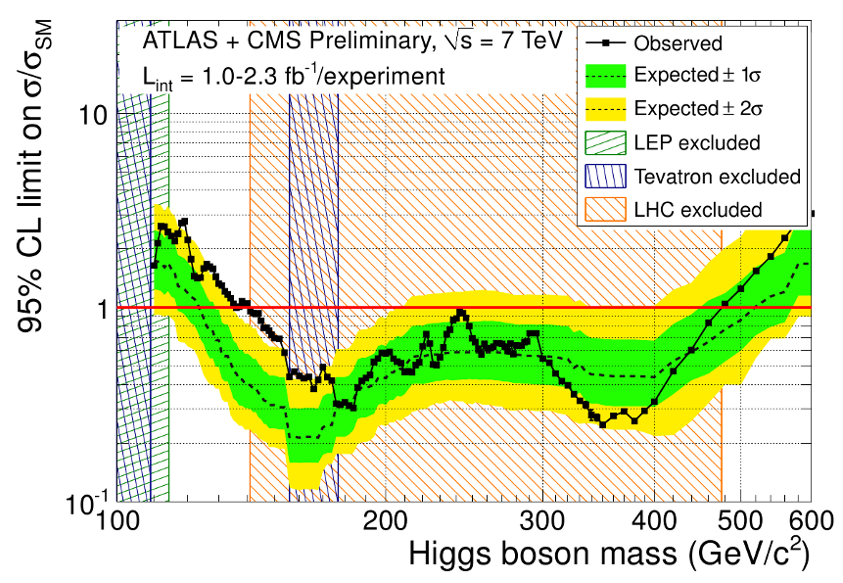
\includegraphics[width=\linewidth]{higgs_limits_alllimits.png}}

\textcolor{red}{Standard Model Higgs boson with 140 $<$ mass $<$ 480~GeV does not exist}

\end{frame}

\begin{frame}
\frametitle{The surviving mass region}

\begin{columns}
\column{0.5\linewidth}
\begin{center}
\vspace{0.25\baselineskip}
LHC direct-search exclusion

\vspace{0.25\baselineskip}
zoomed into 100--200~GeV

\vspace{0.5\baselineskip}
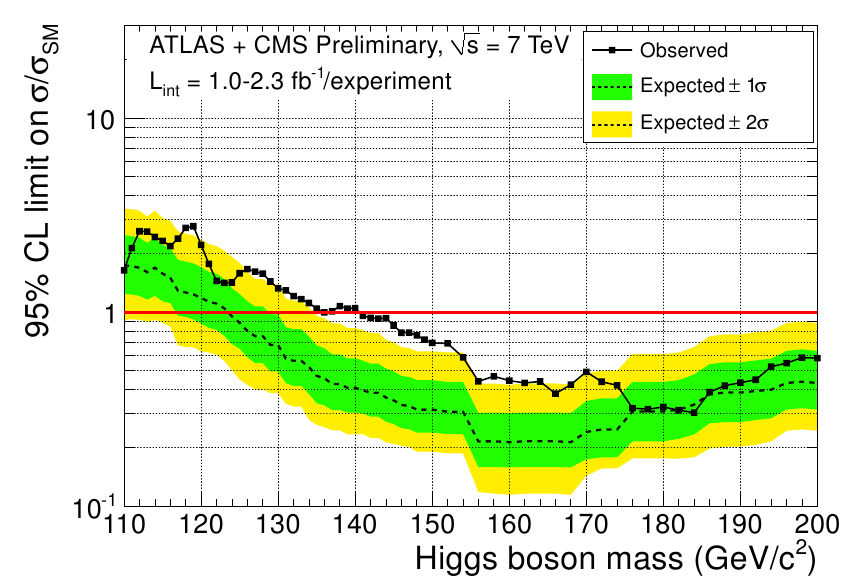
\includegraphics[width=\linewidth]{higgs_limits_zoom.png}
\end{center}

\column{0.5\linewidth}
\begin{center}
Limits inferred from precision Standard Model measurements

($W$, $Z$, top masses, etc.)

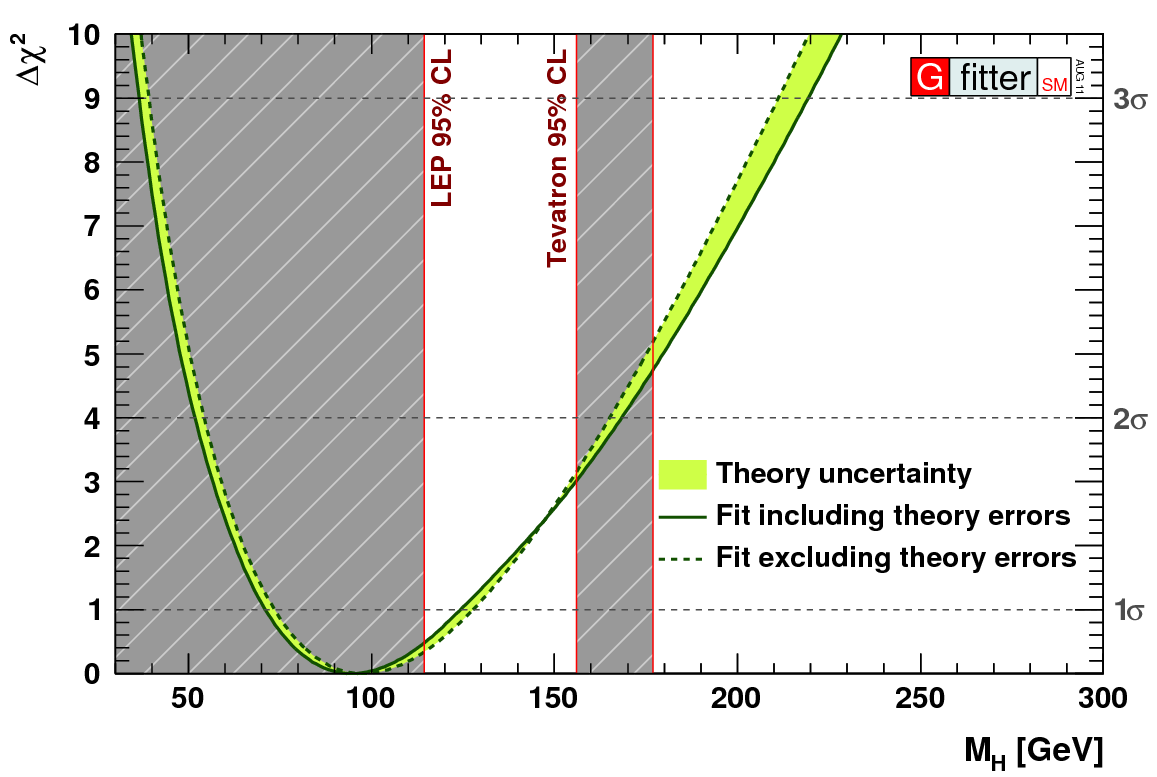
\includegraphics[width=\linewidth]{higgs_limits_indirect.png}
\end{center}
\end{columns}

\begin{itemize}
\item \textcolor{red}{A low-mass Higgs (114--140~GeV) has {\it not} been excluded}
\item This region is also considered most likely by \mbox{precision measurements\hspace{-1 cm}}
\item The slight excess of 110--175~GeV events is not statistically compelling, but it is an excess

%% \only<1>{\item It is also the most difficult:
%% \begin{itemize}
%% \item Higgs $\to$ two $b$ quarks, which looks just like a common process
%% \item Higgs $\to$ two photons, which is extremely rare
%% \item Higgs $\to$ two $\tau$ leptons, which are a little of both
%% \end{itemize}}
%% \only<2>{\item But not impossible!
%% \begin{itemize}
%% \item New techniques (use higher momentum of Higgs $b$ quarks)
%% \item The dataset continues to grow rapidly
%% \end{itemize}
%% \item We are in the endgame of the Higgs search}

\end{itemize}
\end{frame}

\begin{frame}

The Standard Model Higgs, if it exists, has been cornered to a narrow range of masses (finally, after at least 30 years of searches!)

\vfill
ATLAS and CMS will make their complete 2011 datasets public on Dec 13 at 8 AM EST; four-experiment combination (CDF, D$\varnothing$, ATLAS, CMS) should be ready by the end of March 2012

\vfill
LHC expected to produce 2--3 times as much data in 2012 as in 2011--- should be enough to fully discover or refute the Standard Model Higgs

\begin{itemize}
\item If discovered, its properties are key to understanding the large gap between Standard Model particle masses and the Planck quantum gravity scale (the Hierarchy Problem)

\item If not discovered, the cornerstone of the Standard Model will have fallen and we'll {\it know} that there's some exotic physics happening
\begin{itemize}
\item maybe non-standard Higgses that are hidden somehow
\item maybe something completely different
\end{itemize}
\end{itemize}
\end{frame}

%% \section*{First section}
%% \begin{frame}
%% \begin{center}
%% \Huge \textcolor{blue}{First section}
%% \end{center}
%% \end{frame}

\begin{frame}
\frametitle{Conclusions}

\begin{center}
It will be an exciting year.
\end{center}

\label{numpages}
\end{frame}

\begin{frame}
\frametitle{http://www.coffeeshopphysics.com}
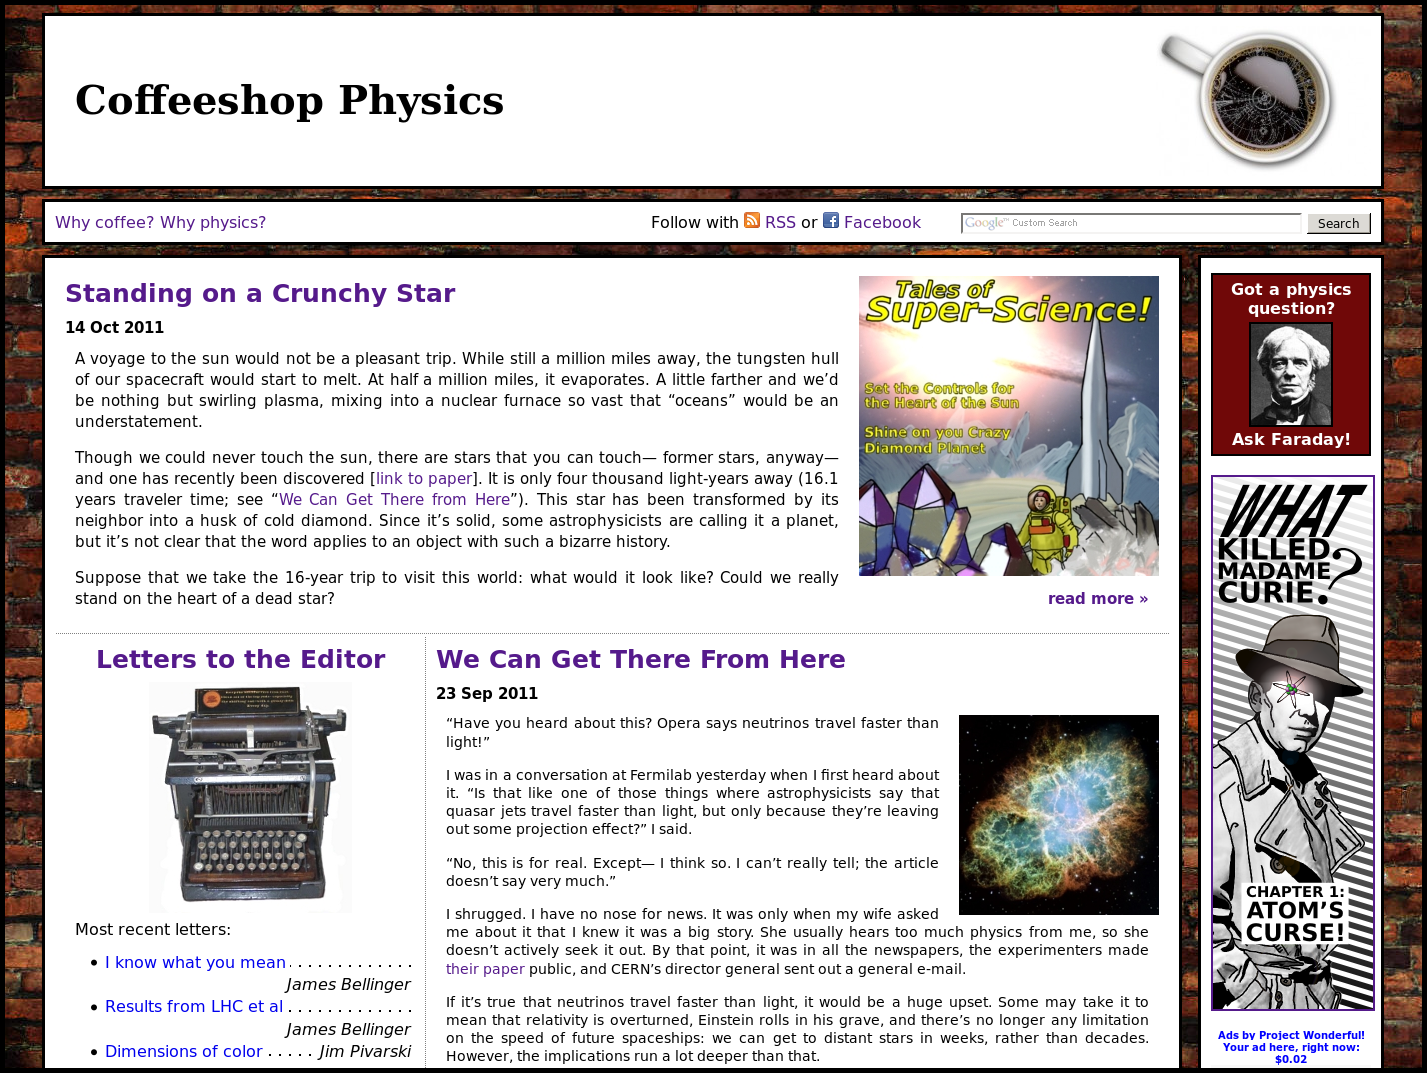
\includegraphics[width=\linewidth]{coffeeshopphysics.png} \hfill
\end{frame}

\end{document}
